In this part we use the methods presented in the theory section to simulate quantum dots with varying complexity. We start with a simple system without interactions, before we gradually move to more complicated systems with a larger number of interacting particles. The main focus is on the comparison between the different trial wave functions and on the study of the various parameters in the model.

\section{Non-interacting particles}
The first step will be to benchmark the different methods on a non-interacting system. For the systems without interactions we know the analytical solution, so they provide us with a good way of testing if the methods work. This way we can also tune the parameters in the models to find parameters that hopefully will give good results when we extend the analysis to interacting particles. The neural network has a lot of flexibility, so a good portion of the chapter will be used to explore its parameter space.  
\\
\\
To get the best convergence possible, it is important that the Markov chains have good convergence properties.  Another important factor in the simulations is the optimization part. Therefore, a good portion of this section will be dedicated to study the convergence of the Markov Chains and the optimization algorithm for Restricted Boltzmann Machines and Neural Networks.
\\
\\
A simple test to check if the methods will be able to produce the desired results is to see if it gives the correct energy when all the variational parameters are set to the known exact values. For the non-interacting case, the optimal variational parameters are known. Since the exact solution are given by the Slater determinant with the single particle wave function, we can simply set the variational parameters so that all other parts of the wave function equals 1. This means that we set all weights in the RBM and the NN equal to 0. This way we get the exponent of 0, which is equal to 1. 
\\
\\
In table \ref{tab:non-interacting 2 particles in 2 dims} the results are shown, and they correspond exactly to the analytical values for all systems. The variance is also zero. This means that the Markov Chain samples are all equal to the exact values. 
\\
\\
The same can be seen for higher number of particles and dimensions. This comes from the fact that the single-particle wave functions are the exact solutions for $\alpha = 1$, so by setting all other parameters to zero, we simply remove those parts of the wave function. The only part left is then the slater determinant which is the exact solution.  

\begin{table}[]
    \centering
    \begin{tabular}{c|c|c|c} 
        Wavefunction & Energy (N=2) & Energy (N=6) & Energy (N=12) \\ \hline
        $\uppsi_\text{SD}$ &  $2.0\pm 0.00$ & $10.0 \pm 0.00$  & $28.0 \pm 0.00$ \\
        $\uppsi_\text{SD}\uppsi_\text{J}$ & 2.0 & 10.0 & 28.0 \\
        $\uppsi_\text{SD}\uppsi_\text{RBM}$ & 2.0 & 10.0 & 28.0 \\
        $\uppsi_\text{SD}\uppsi_\text{NN}$ & 2.0 & 10.0 & 28.0\\ \hline
        Exact & 2.0 & 10.0 & 28.0 \\
    \end{tabular}
    \caption{Ground state energy for different combinations of wavefunctions, for a system of N non-interacting particles in 2 dimensions. The variance is zero for all the energy estimates.}
    \label{tab:non-interacting 2 particles in 2 dims}
\end{table}

\subsection{Convergence properties}
As we saw in the last part, all methods are able to reproduce the exact values when the optimal parameters are known. However, it is important that it is able to find those optimal values as well. To get good estimates of the gradients and the actual local energy, a good Markov Chain is needed. To study the chains we therefore need to study the chain when the variational parameters are not set to the exact values. This is because for the exact values, the variance is zero and we get no useful information about the different parameters in the simulation. 
\\
\\
To get accurate results, it is important that the Markov chain converge properly. Therefore, we will use some time to study how the chains reacts to different parameters, and find the best ones. This will vary from system to system, so it is important to do a proper search for parameters for all systems. The focus in this chapter will be on studying the parameters for the RBM and the NN. 
\\
\\
Both importance sampling and brute force sampling will be studied. 
First, the chain will be studied by looking at plots of the local energy, and see how it varies for different parameters. We will also look at the variance in the Markov Chain, as well as the acceptance ratio. 
\\
\\
One simple method to check the convergence is to look at a trace-plot of the values obtained in the chain. Typically, we want the chain to stabilize around a value, but still oscillate around that value. This means that we want good mixing.

\subsubsection{Slater}
The first system we will study is the wave function consisting of a simple Slater determinant. We expect it to find the exact values, since the single particle wave functions are the exact solution. We will start by studying the brute-force sampling method to find the optimal step-length. 

\subsubsection{Slater-Jastrow}
Again, we will start by studying the effect of the step-length in the brute-force Metropolis algorihtm. 

Next, the results from changing the brute-force proposals with importance-sampling is shown in figure \ref{} and table \ref{}. 

\subsubsection{Slater-RBM}
Now we will look at the system with a wave function consisting of a slater determinant and a restricted boltzmann machine. The results are shown in figure \ref{fig:rbm_mcmc_diagnostic} and table \ref{tab:rbm_mcmc_diagnostic}. 

\begin{figure}[h!]
    \centering
    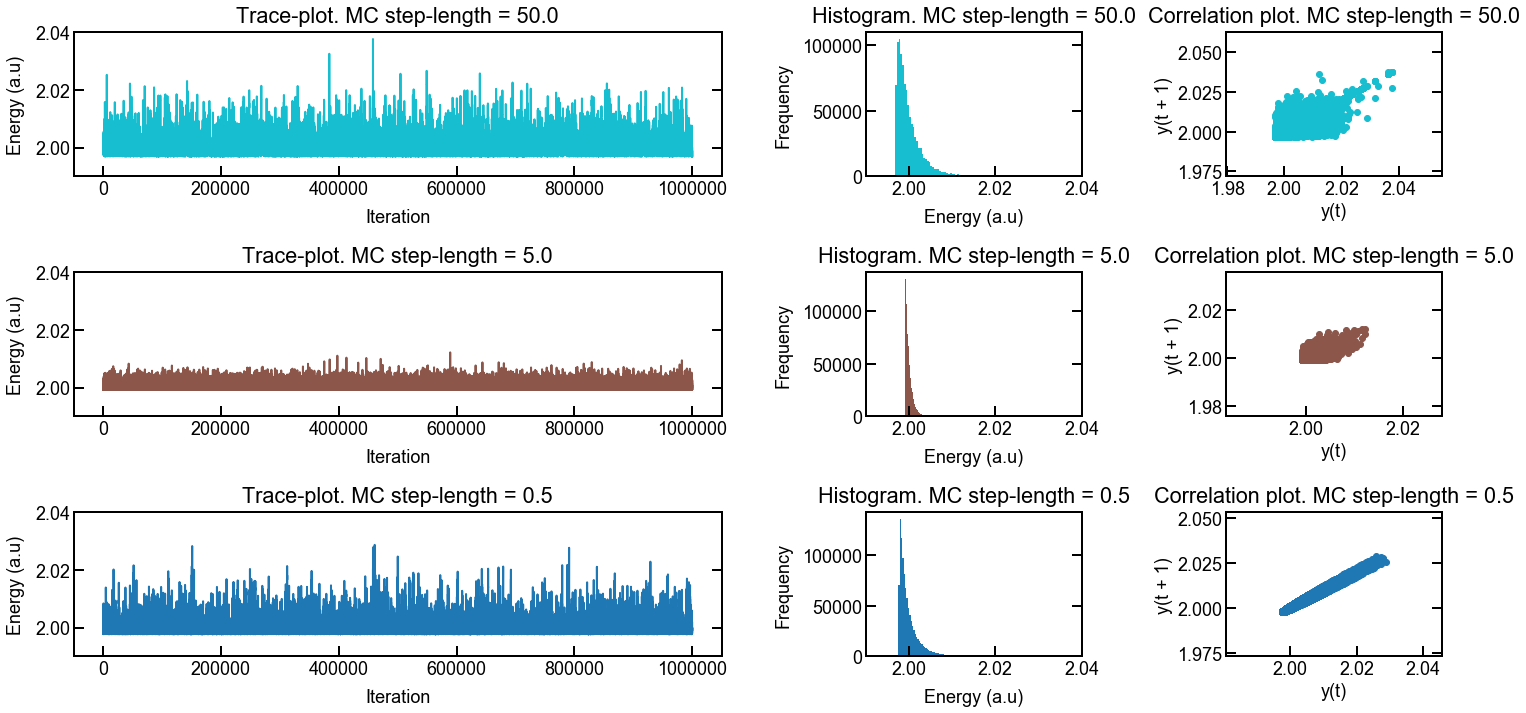
\includegraphics[width=\textwidth]{test.png}
    \caption{Various diagnostic plots for MCMC. The system is a Slater-RBM wave function for non-interacting particles with 2 particles in 2 dimensions.}
    \label{fig:rbm_mcmc_diagnostic}
\end{figure}

\begin{table}[h!]
    \centering
    \begin{tabular}{rrrr}
     MC step-length &    Energy &           Var &  Acceptance ratio \\ \hline
                0.5 &  1.999973 &  2.409328e-09 &          0.930229 \\
                5.0 &  1.999999 &  1.873899e-11 &          0.434517 \\
               50.0 &  1.999986 &  2.214887e-09 &          0.045164 \\
    \end{tabular}
    \caption{The system is a Slater-RBM wave function for non-interacting particles with 2 particles in 2 dimensions.}
    \label{tab:rbm_mcmc_diagnostic}
\end{table}
The first thing to note is the trace-plots. All methods have relatively good mixing properties, and they converge to the target distribution immediately. However, the chain for a MC step-length of 0.5 seems to have a much lower variance, and the values are more spot on. This can also be seen in table \ref{}. The variance is an order of 2 lower. When studying the chains, we are also interested in looking at the correlation between the samples. For $\detla x = 5.0$, the samples are clearly highly correlated. The reason for this is possibly that we propose new position that are to different from the last step, many proposals will then be rejected, and we will stay in the same position multiple steps. Choosing the step-length smaller seems to give less correlated. However, when choosing it to small the samples seems to be more correlated again. This can be seen from the correlation plot for $\delta x = 0.05$. 
\\
\\
We can now compare it to the results from using importance sampling instead of the brute-force sampling. 
\\
\\
In figure \ref{} and table \ref{}, the results are shown for different step sizes. 
\\
\\
For the Boltzmann machine we have som extra flexibility compared to the standard Slater and Slater-Jastrow wavefunctions. the number of nodes in the hidden layer can play an important role in the accuracy of the estimates. We will now use importance sampling with step-length = ... for the rest of the analysis, and compare the convergence for different number of hidden nodes.  
\subsubsection{Slater-NN}
As before, we will start by studying the step-length of the brute-force proposal algorithm before we look at importance sampling. The same steps as for the RBM will be conducted to test different step-lengths. 
\\
\\
The results are shown in 
\subsubsection{Brute Force Metropolis}
Looking at the trace-plots in figure \ref{}, we note that a step-length of ... seems to give good properties. For ... and ..., the chain gets stuck on certain values for a longer period of time, which restricts the chain from exploring other values. In table \ref{} the variance are shown, together with the ... 
\subsubsection{Importance Sampling Metropolis}
As for the brute-force method
\subsection{Optimization}
When the Markov Chain converges properly and produces accurate gradients and local energies, the next step is to find the optimal way to actually update the variational parameters of the model.  Again, this will depend on the system. The standard gradient descent and the adam algorithm will be compared for varying parameters.
\subsubsection{Gradient descent}
In this section the convergence of the gradient descent method is studied. In figure \ref{} the results for different learning rates are shown. 
\subsubsection{Adam}
\subsection{Energy}
Now that the optimal parameters and methods are found, they will be used to calculate the energy of a system of non-interacting particles. The analytical results is used as a benchmark for the methods.
\\
\\
For the non-interacting system, we assume to get very got results for every combination of the Wavefunction elements. The results from running 50 optimization steps with $10^5$ Monte Carlo steps in each iteration are shown in table:
\begin{table}[h!]
\centering
\begin{tabular}{c|c}
    Wavefunction & $\psi_{SD}\psi_{J}$  \\
    Test &  Test \\
\end{tabular}
\end{table}
We see that all wavefunction gives accurate results for the non-interacting case. 

\subsection{Electron density}
We can now study the electron density to see where the particles tends to be. 

\section{Interacting particles}
In this section systems of interacting particles in a quantum dot are studied. We no longer have easily obtained analytical expression, except for certain cases. We will mainly test over method against the system where the analytical solution are found. Our implementation is compared to previous work done on similar systems. The most interesting part is to see how the neural network compares to the restricted Boltzmann Machine. 
\\
\\
We now also want to combine all wavefunction elements to see if it is possible to get even closer to the exact value. It is interesting to see if the neural network are able to improve the results given by the rbm. This will be done by training each part separately. First, we find the optimal parameter with only the slater. Then we add the rbm and trains that. Then, we add the neural network and trains that separately as well. The results are shown in table \ref{} and figure \ref{}. 

\newpage